\subsection{Thermal Conductivity Sensitivity Validation}\label{sec:conductivity}
The thermal conductivity, $K_{th}$ of geologic repository host media impacts 
the speed of transport, and therefore the time evolution of thermal energy 
deposition, in the medium. 

\FloatBarrier
\subsubsection{LLNL Model Results}
In the creation of the \gls{STC} database, the thermal conductivity was varied 
across a broad domain for each isotope, $i$, package spacing, $s$, limiting 
radius $r_{calc}$, and thermal diffusivity $\alpha_{th}$, considered.  By 
varying the thermal conductivity of the repository model from 0.1 to 4.5
$[W\cdot m^{-1} \cdot K^{-1}]$, this sensitivity analysis succeeds in capturing the domain of 
thermal conductivities witnessed in high thermal conductivity salt deposits as 
well as low thermal conductivity clays.

\begin{figure}[htbp!]
\begin{center}
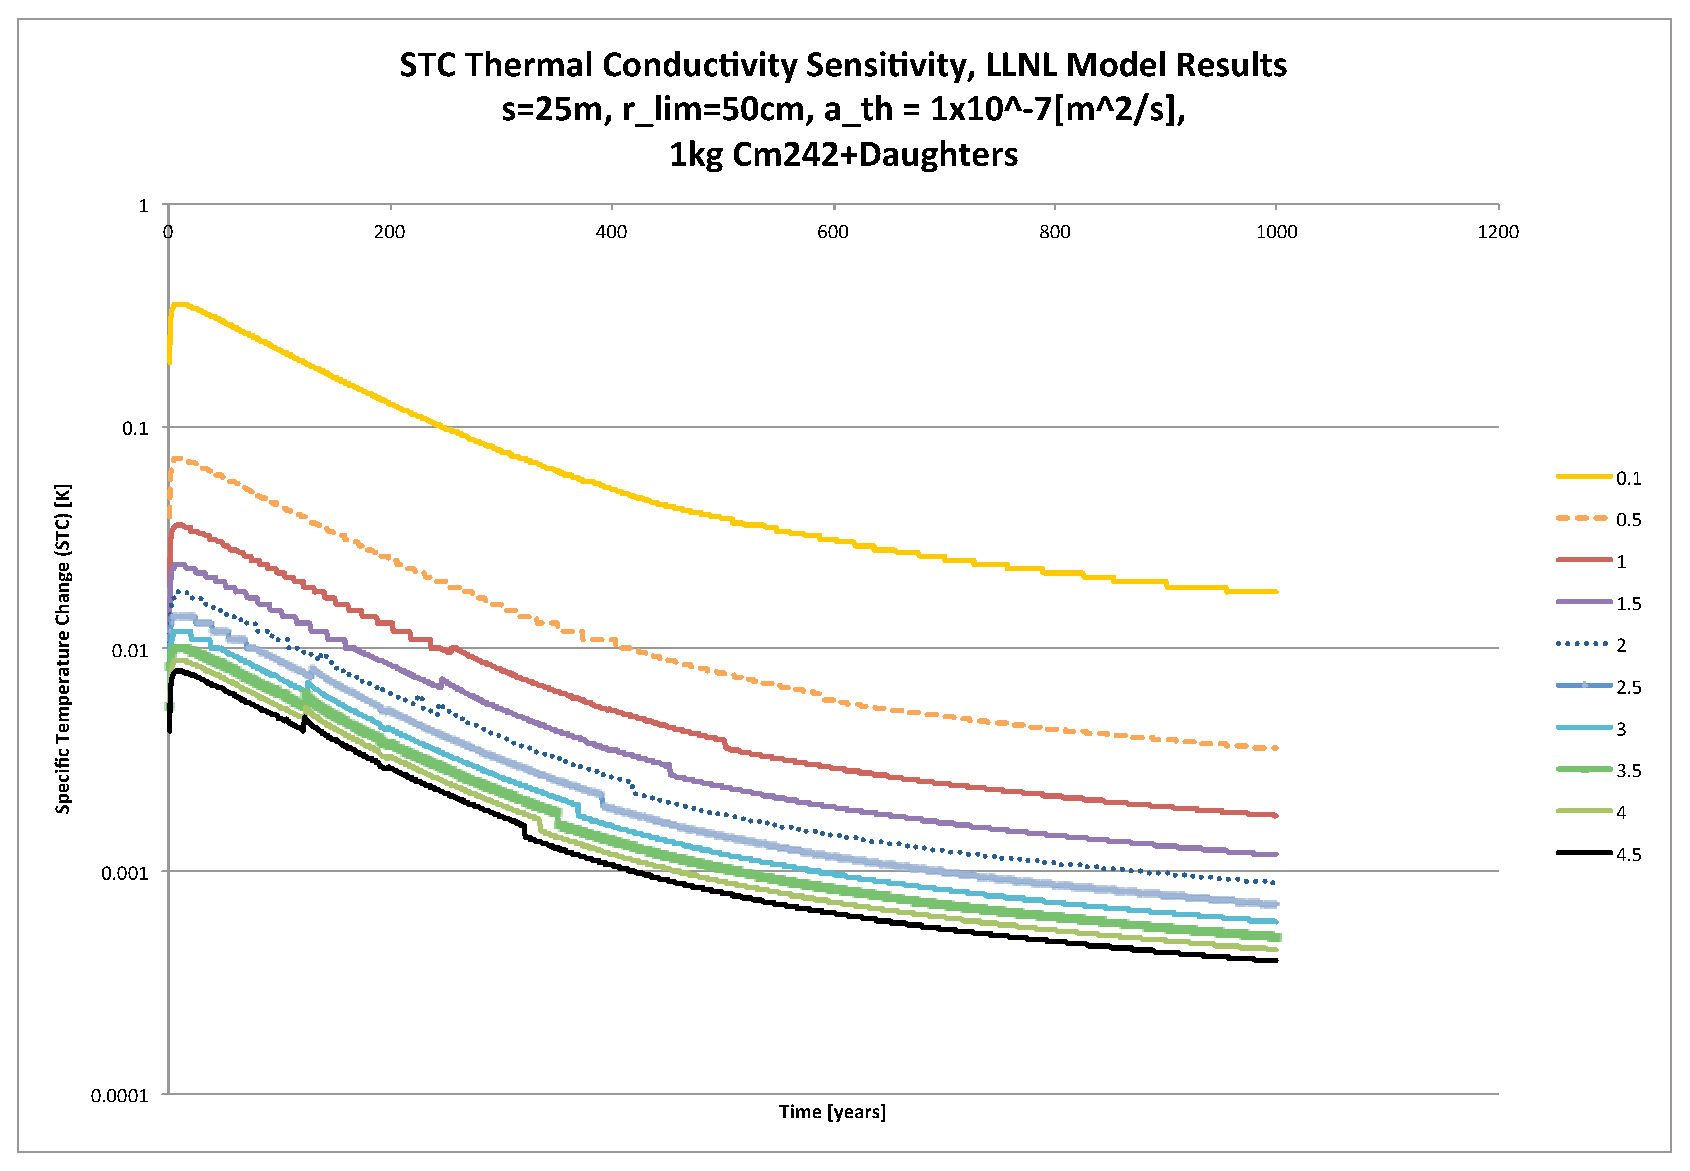
\includegraphics[width=0.7\textwidth]{./chapters/demonstration/conductivity/Cm242kth_alpha_low.eps}
\end{center}
\caption[$K_{th}$ Sensitivity for Low $\alpha_{th}$ in LLNL Model]{Increased thermal conductivity decreases thermal energy deposition 
(here represented by \gls{STC}) in the near field (here $r_{calc} = 0.5 m$).}
\label{fig:Cm242Kth_alpha_low}
\end{figure}

Figure \ref{fig:Cm242Kth_alpha_low} shows the trend in which increased thermal conductivity of a medium decreases thermal energy 
deposition in the near field. This indicates, then that thermal conductivity is 
an important parameter for repository geologic medium selection. 

\FloatBarrier
\subsubsection{Cyder Results}

In a similar analysis, the thermal conductivity was compared both with the 
spacing between waste packages and the limiting radius. 

Figures \ref{fig:kr} and \ref{fig:ks} validate the trend noted above that 
increased thermal conductivity of a medium decreases thermal energy deposition 
in the near field.  Additionally, analysis with the \Cyder STC database 
demonstrates the way in which the importance of spacing and the importance of 
the limiting radius decrease with increasing $K_{th}$.

\begin{figure}[htbp!]
\begin{center}
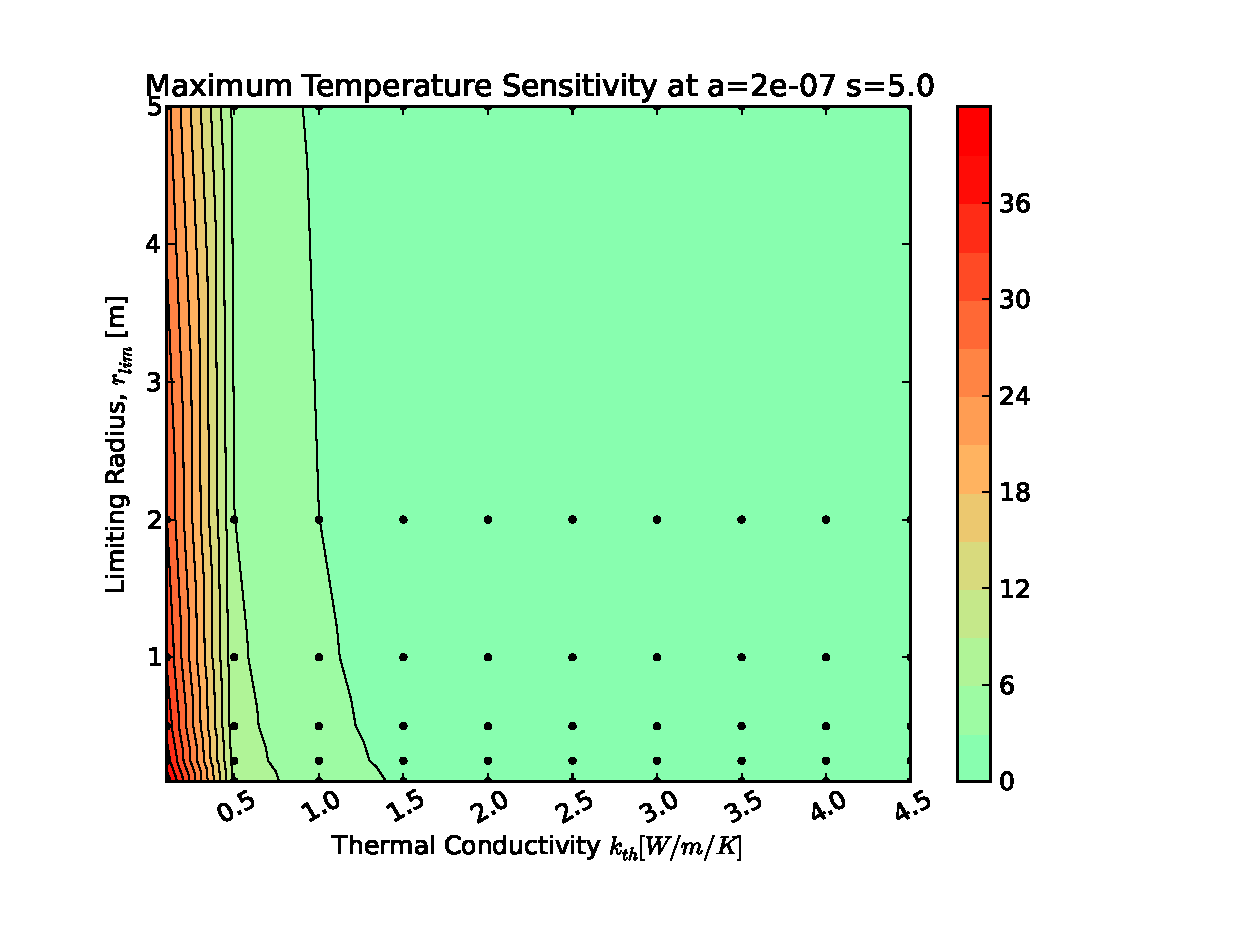
\includegraphics[width=0.7\textwidth]{./chapters/demonstration/conductivity/kr.eps}
\end{center}
\caption[$K_{th}$ vs. $r_{lim}$ Sensitivity in Cyder]{\Cyder results agree with 
those of the LLNL model. The importance of the limiting radius decreases with 
increased $K_{th}$. The above example thermal profile results from 10kg of 
$^{242}Cm$}
\label{fig:kr}
\end{figure}

\begin{figure}[htbp!]
\begin{center}
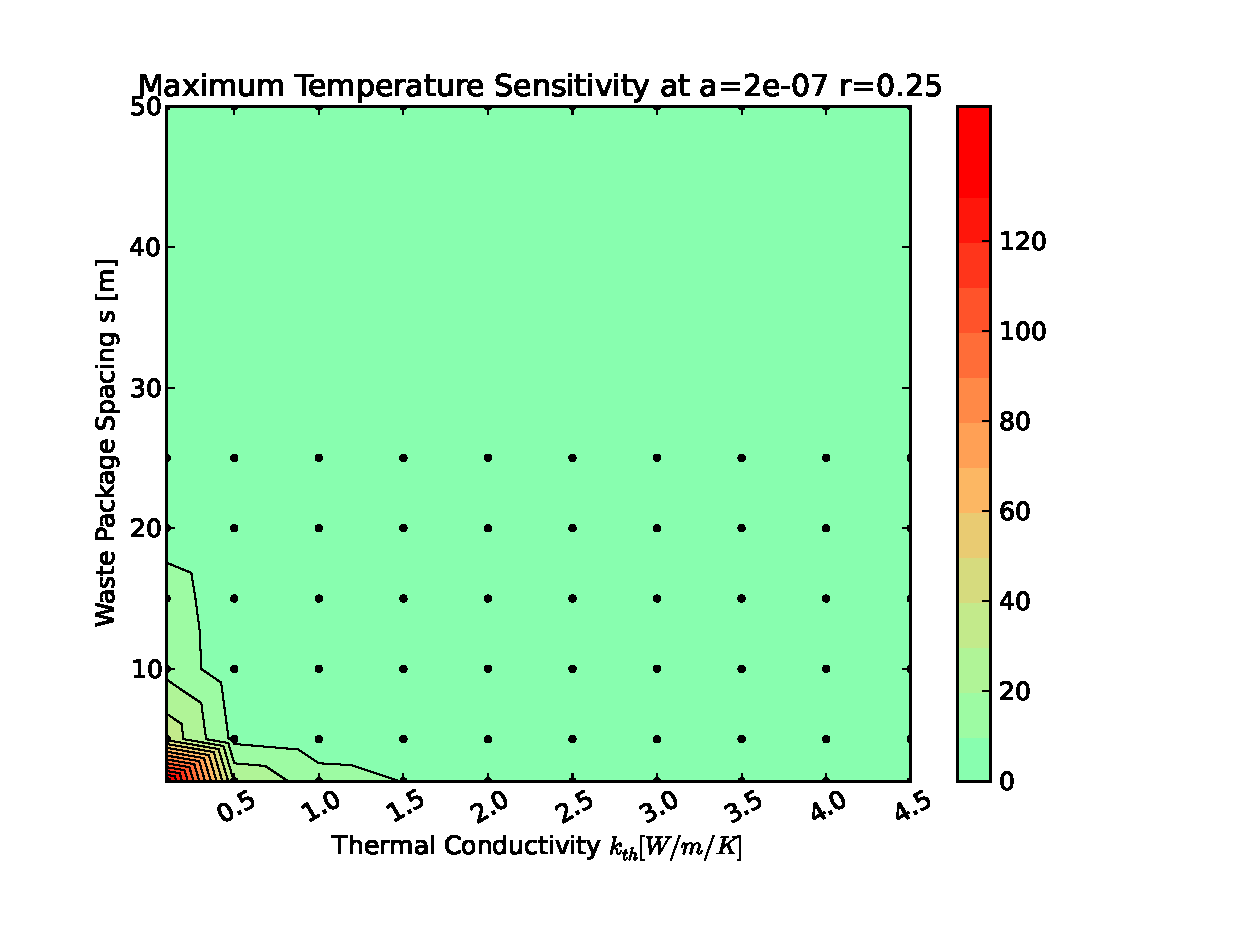
\includegraphics[width=0.7\textwidth]{./chapters/demonstration/conductivity/ks.eps}
\end{center}
\caption[$K_{th}$ vs. Waste Package Spacing Sensitivity in Cyder]{Cyder results agree with 
those of the LLNL model. The importance of the limiting radius decreases with 
increased $K_{th}$. The above example thermal profile results from 10kg of 
$^{242}Cm$}
\label{fig:ks}
\end{figure}


